\documentclass[twocolumn]{article}

\usepackage{scrextend}
\changefontsizes{8pt}

\makeatletter
\renewcommand*{\fps@figure}{!htb}
\renewcommand*{\fps@table}{!htb}
\makeatother

\usepackage{sectsty}
\sectionfont{\fontsize{11}{11}\selectfont}
\subsectionfont{\fontsize{10}{11}\selectfont}

\usepackage[compact]{titlesec}
\titlespacing{\section}{0pt}{2ex}{1ex}
\titlespacing{\subsection}{0pt}{1ex}{1ex}
\titlespacing{\subsubsection}{0pt}{0.5ex}{1ex}

\setlength{\parskip}{0cm}
\setlength{\parindent}{1em}

\usepackage{geometry}
 \geometry{
 a4paper,
 total={170mm,257mm},
 left=20mm,
 top=20mm,
 }
\usepackage[utf8]{inputenc}
\usepackage[hidelinks]{hyperref}
\usepackage{amsmath, bm}
\usepackage[ruled,vlined]{algorithm2e}
\usepackage{amssymb}
\usepackage{graphicx}
\usepackage{float}
\usepackage{booktabs}
\usepackage[parfill]{parskip}
\usepackage{comment}
\usepackage{subcaption}
\usepackage{booktabs}



\usepackage{listings}
\lstset{
    language=Python,
    breaklines=true,
    breakatwhitespace=true,
    basicstyle=\footnotesize,
    frame=lines
}
\usepackage[capitalise, nameinlink]{cleveref}

\usepackage[sorting=none, style=verbose]{biblatex}
\addbibresource{lab_7.bib}

\usepackage{titling}
\setlength{\droptitle}{-1cm}

\title{\Large COMP6248 Lab 8 Exercise -- Exploring Latent Spaces}
\author{\small Wei Chien Teoh (Eugene)\\\bigskip \href{mailto:wct1c16@soton.ac.uk}{wct1c16@soton.ac.uk}}
\date{\small 29 April 2021}

\begin{document}

\maketitle

\section*{Introduction}

The results are seeded using \lstinline{pytorch_lightning.seed_everything(0)} to provide reproducible results.

\section{Exploring the latent space of a VAE}

\subsection{Systematically sample a VAE}

\begin{lstlisting}[caption={Code to generate latent image.}]
    latent_img = np.empty((588, 588))

    x_points = np.linspace(-4, 4, 21)
    y_points = np.linspace(-4, 4, 21)
    xx, yy = np.meshgrid(x_points, y_points)
    for i in range(len(xx)):
        for j in range(len(yy)):
            z = torch.tensor([xx[j, i], yy[j, i]], dtype=torch.float32).view(1, 2)
            output = dec(z)
            img = output.view(28, 28).detach().numpy()
            latent_img[j*28:j*28+28, i*28:i*28+28] = img
\end{lstlisting}

\begin{figure}
    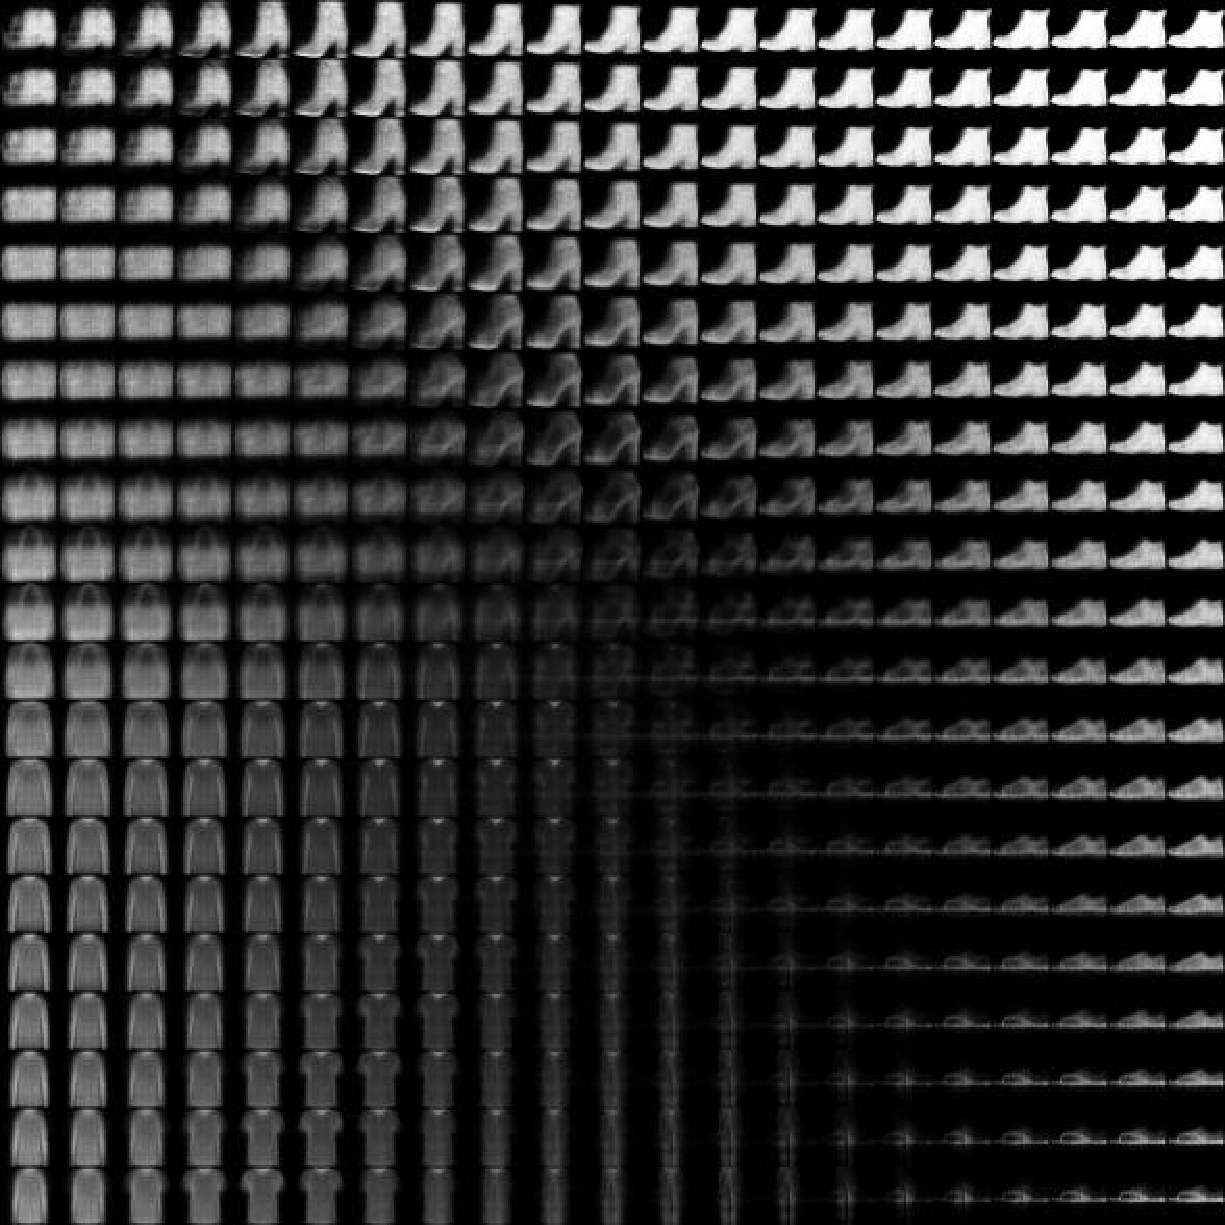
\includegraphics[width=\linewidth]{Figures/latent_img.pdf}
    \caption{Latent image of VAE.}
    \label{fig:latent-img}
\end{figure}

\section{Exploring the code space of a standard auto-encoder}

\subsection{Systematically sample an Autoencoder}

\begin{figure}
    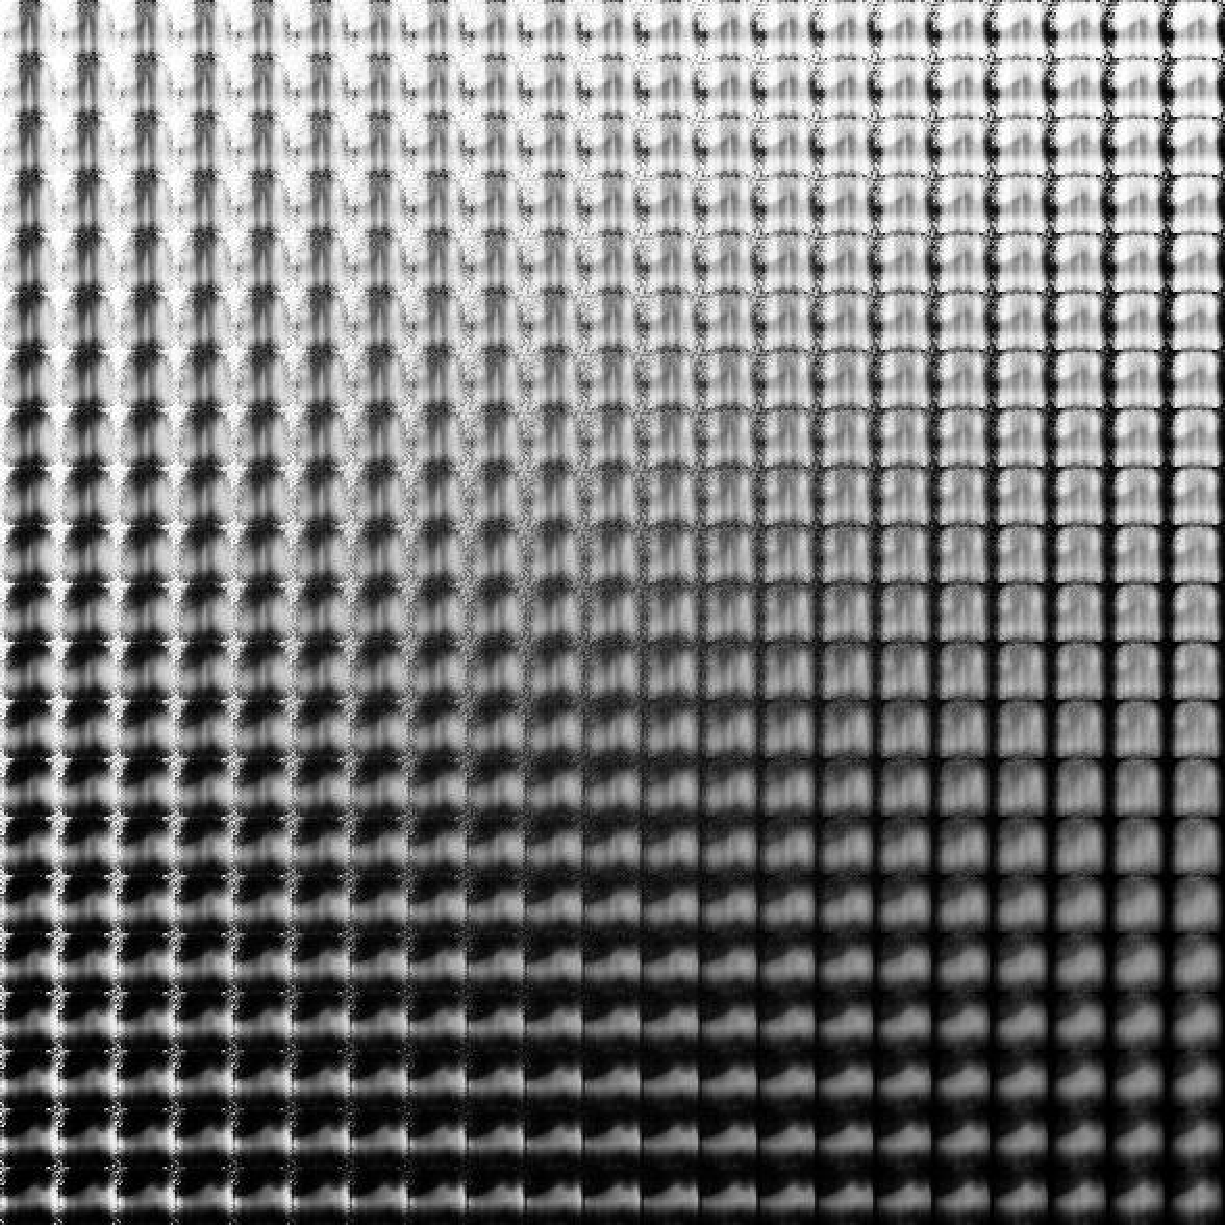
\includegraphics[width=\linewidth]{Figures/latent_img_2.pdf}
    \caption{Latent image of autoencoder.}
    \label{fig:latent-img-2}
\end{figure}

\subsection{Compare the latent spaces of the VAE and autoencoder}

\cref{fig:latent-img} shows that VAE is able to learn latent representations of the data such as the structure of shirts, boots, pants, etc. The VAE also attempts to learn orthogonal/uncorrelated structures because of the orthogonality (non-diagonals are zeros) imposed while learning the latent variance.

\cref{fig:latent-img-2} rather shows that the autoencoder performs compression of the data into a smaller subspace, thus learning the most important latent features. It can be observed that the latent representations are composed of a linear combination of the structures such as shirts, boots, pants, etc.

\end{document}